\section{Gets and Multi-gets (90 pts)\label{sec:5}}

    In this section the system is analyzed for mixed workloads whereby SET requests and GET requests are in the ration
    1:1 but for GET the amount of keys requested is increased in addition to the middleware possibly splitting up GET
    requests with multiple keys fairly to each \srv{}s. The experiment aims to find out under what conditions this
    splitting, also called \emph{sharding} is preferable and how the throughput changes amongst differently sized GET
    requests. In table \ref{tab:50_setup} the experimental setup is documented.

    The experiment intends to use the most performant middleware as such the correct number of worker threads needs to
    be inferred for the case of 12 total clients. This experiment has two limiting factors:
    \begin{itemize}
        \item GET requests are network bound on the end of each \srv{}. The number of requests is expected to go down
              for more keys as replies get larger.
        \item SET requests are network bound on the end of each \cli{}. The number of requests is expected to not change
              as SETs are of fixed size.
    \end{itemize}
    From experiment \ref{sec:4} it becomes clear that there is no significantly measurable performance impact using more
    worker threads than is required for clients. This means that any amount of worker threads beyond 8 is appropriate to
    use for this experiment for SETs. Experiment \ref{sec:3} is of minimal use as only single \srv{} configurations were
    tested. Yet it can be deduced that the middleware can handle at least one \srv{}s load of single-key GET replies
    without any problems. As no significantly measurable performance impact for SETs exist and multi-key GET requests
    are not yet observed with three \srv{}s active the decision was made to use 64 worker threads to exclude any
    performance impacts possible due to too little threading on the middleware.

    Important in this section's data is the exclusion of the 60s stable-phase window as histograms are used. As memtier
    reports histograms for the complete run and not a configurable stable window this decision was made to allow
    comparing not only data from the middleware and memtier but also relate it to histograms.

    \begin{table}
        \scriptsize{
            \begin{tabular}{|l|c|}
                \hline Number of servers                & 3 \\
                \hline Number of client machines        & 3 \\
                \hline Instances of memtier per machine & 2 \\
                \hline Threads per memtier instance     & 1 \\
                \hline Virtual clients per thread       & 2 \\
                \hline Workload                         & ratio=1:$<$Multi-Get size$>$ \\
                \hline Multi-Get behavior               & Sharded (5.1) and Non-Sharded (5.2) \\
                \hline Multi-Get size                   & [1, 3, 6, 9] \\
                \hline Number of middlewares            & 2 \\
                \hline Worker threads per middleware    & 64 \\
                \hline
            \end{tabular}
        }
            \caption{Experimental parameters for experiments 5.1 and 5.2.\label{tab:50_setup}}
    \end{table}a single key, whereas this is not the case for the sharded case.

    \subsection{Sharded Case\label{subsec:5_sharded}}

        \begin{figure*}
            \vspace*{-.5\baselineskip}
                \centering
            \begin{subfigure}[t!]{0.43\textwidth}
                \centering
                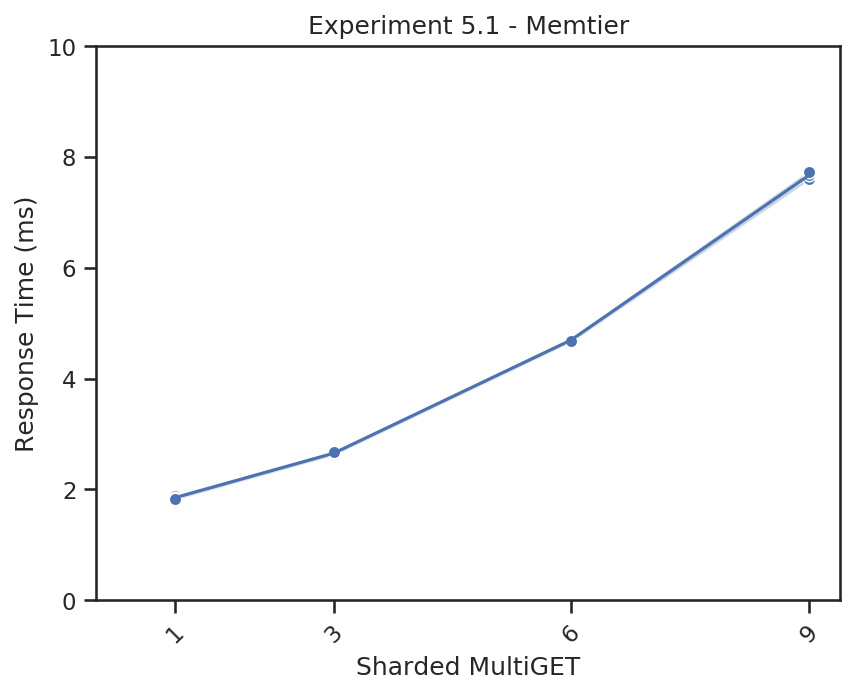
\includegraphics[width=\textwidth]{../data_analysis/figures/5-1_mt_response-time.png}
                \caption{Average response times.\label{fig:shard_mt_rt}}
            \end{subfigure}
            \begin{subfigure}[t!]{0.56\textwidth}
                \centering
                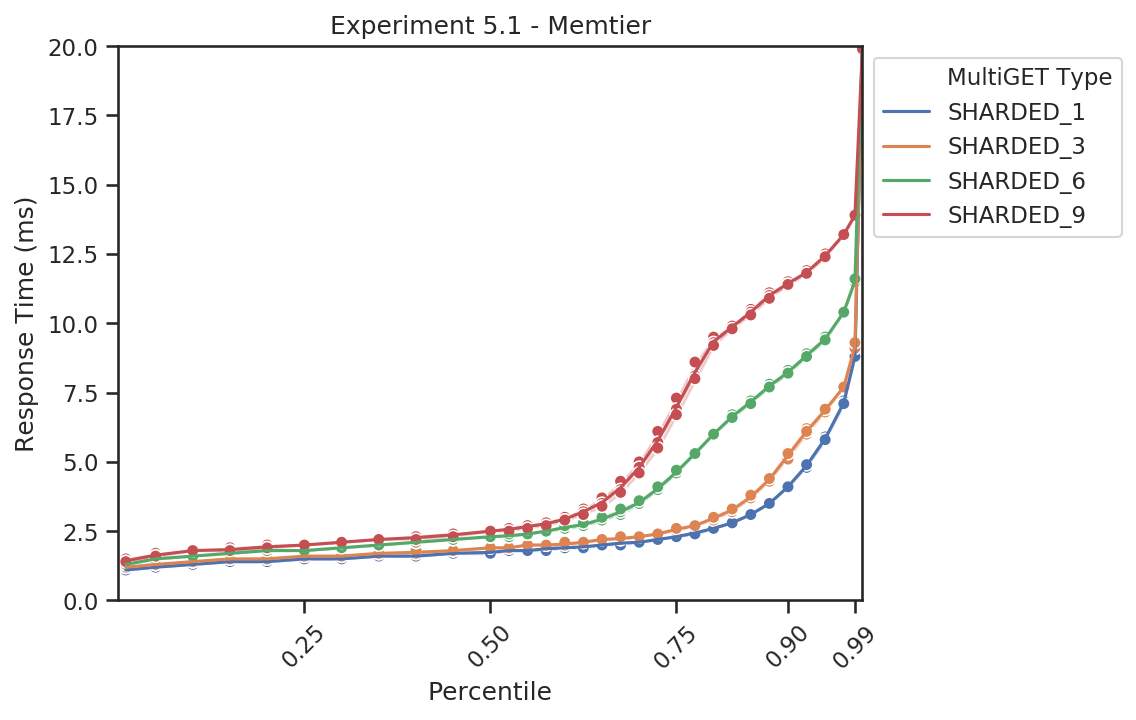
\includegraphics[width=\textwidth]{../data_analysis/figures/5-1_mt_percentiles.png}
                \caption{Percentiles of all response times.\label{fig:shard_mt_rt_percentiles}}
            \end{subfigure}
            \caption{Response times measured on \cli{}s. The graphs include error bars and represent response times
            for GET packets using sharded behaviour on the \mw.\label{fig:shard_mt}}
        \end{figure*}

        \begin{figure*}
            \vspace*{-.5\baselineskip}
                \centering
            \begin{subfigure}[t!]{0.48\textwidth}
                \centering
                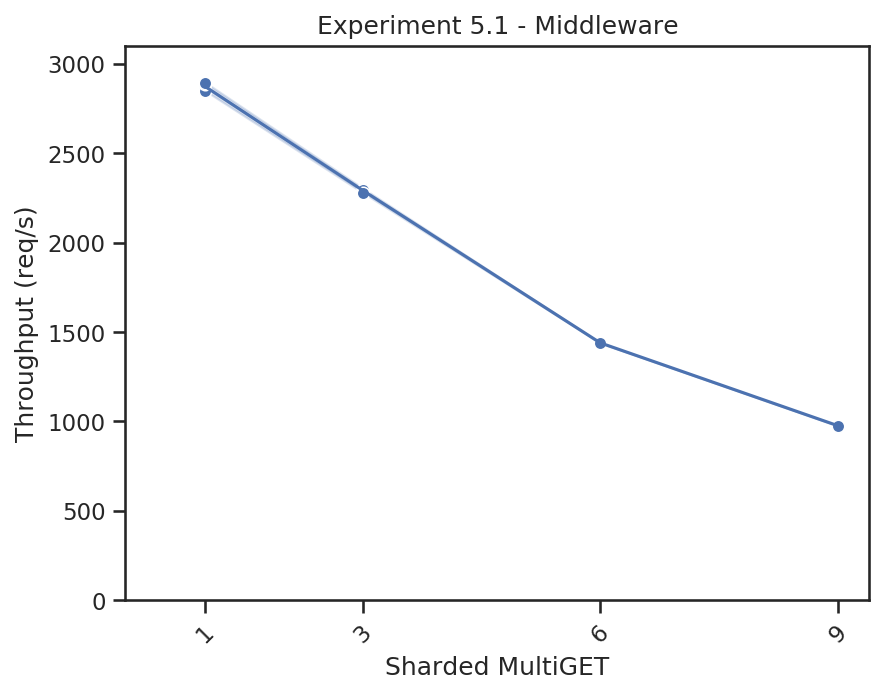
\includegraphics[width=\textwidth]{../data_analysis/figures/5-1_mw_thoughput.png}
                \caption{Request throughput.\label{fig:shard_mw_tp}}
                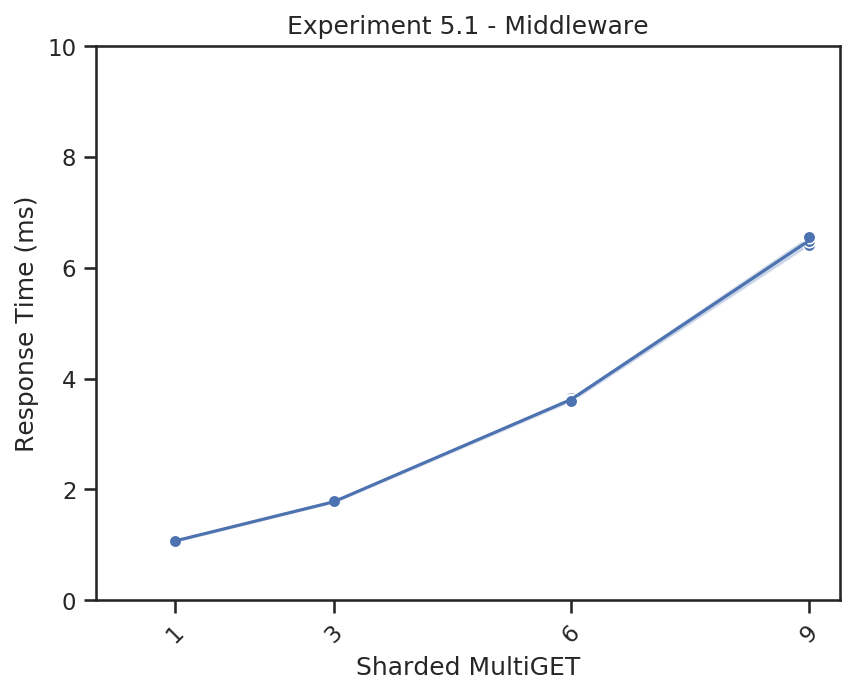
\includegraphics[width=\textwidth]{../data_analysis/figures/5-1_mw_response-time.png}
                \caption{Response times.\label{fig:shard_mw_rt}}
            \end{subfigure}
            \begin{subfigure}[t!]{0.48\textwidth}
                \centering
                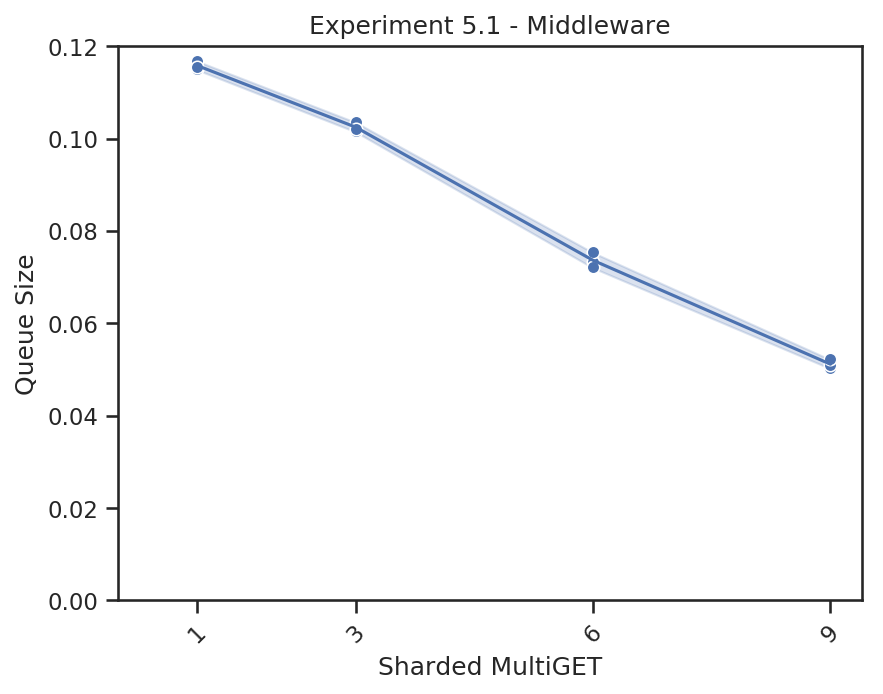
\includegraphics[width=\textwidth]{../data_analysis/figures/5-1_mw_queue-size.png}
                \caption{Queue sizes.\label{fig:shard_mw_qs}}
                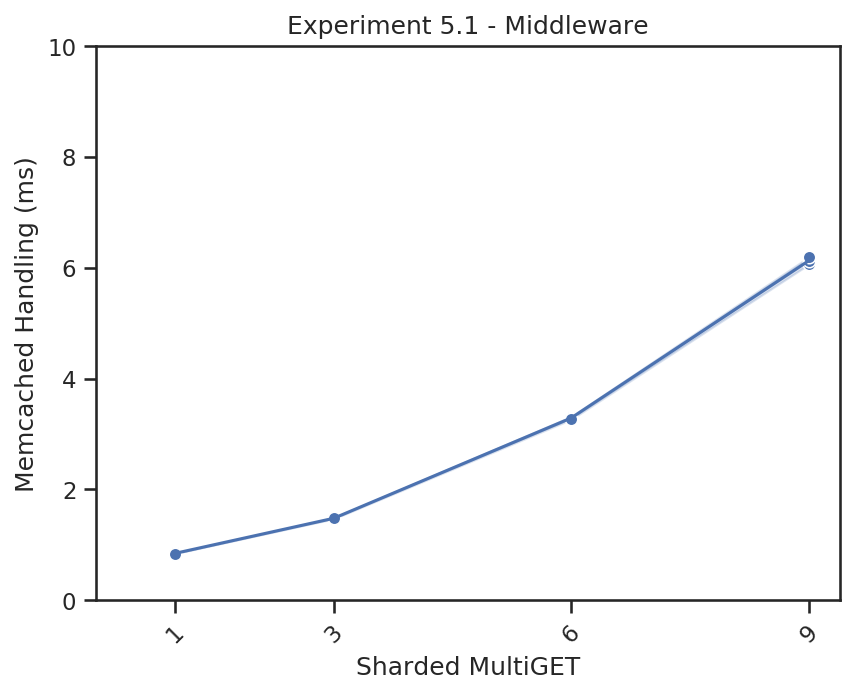
\includegraphics[width=\textwidth]{../data_analysis/figures/5-1_mw_mc-comm-time.png}
                \caption{Memcached communication time.\label{fig:shard_mw_mct}}
            \end{subfigure}
            \caption{\mw{} statistics based on GET requests. Requests are defined as consisting of one GET request
                     followed by a variable amount of keys to be requested.\label{fig:shard_mw}}
        \end{figure*}

        \subsubsection{Explanation\label{subsubsec:5_sharded_summary}}

            As can be seen in the subfigures of figure \ref{fig:shard_mt} the more keys are requested in a single GET
            request the larger the average response becomes. There is a rough linear behaviour in increasing response
            times for larger keys which is expected. Also it is of interest to note the stability of the response times;
            the system looks to be working optimally without outside interference.

            The distribution of percentiles at the 50-percentiles don't match for requests with 6 and 9 keys well. The
            75-percentiles do on the other hand. This is an indication that the distribution has multiple peaks to
            different degrees. This agrees with the histograms obtained (see figure \ref{fig:histogram_sharded_mw}).
            Even though differently sized GET requests are not easily comparable their percentiles grow in a similar
            fashion. This shows their distributions are all based on the same base model though.

            For all requests the queue in the middleware is almost always empty. This shows the middleware performing
            well in terms of request handling. The hypothesis is therefore the middleware must be spending lots of time
            on the communication and packet handling with memcached. Figure \ref{fig:shard_mw_mct} visualizes the
            average communication and packet handling time per key size. Comparing the graph with figure
            \ref{fig:shard_mt_rt} the hypothesis is verified. A discussion comparing this behaviour with no sharding
            follows in subsection \ref{subsec:5_summary}.\newline
            The throughput reported by the middleware in figure \ref{fig:shard_mw_tp} shows a downwards trend for
            requests processed. This is expected as even though fewer requests are made, the throughput in keys
            requested increases.

    \subsection{Non-sharded Case\label{subsec:5_nonsharded}}

        \begin{figure*}
            \vspace*{-.5\baselineskip}
                \centering
            \begin{subfigure}[t!]{0.43\textwidth}
                \centering
                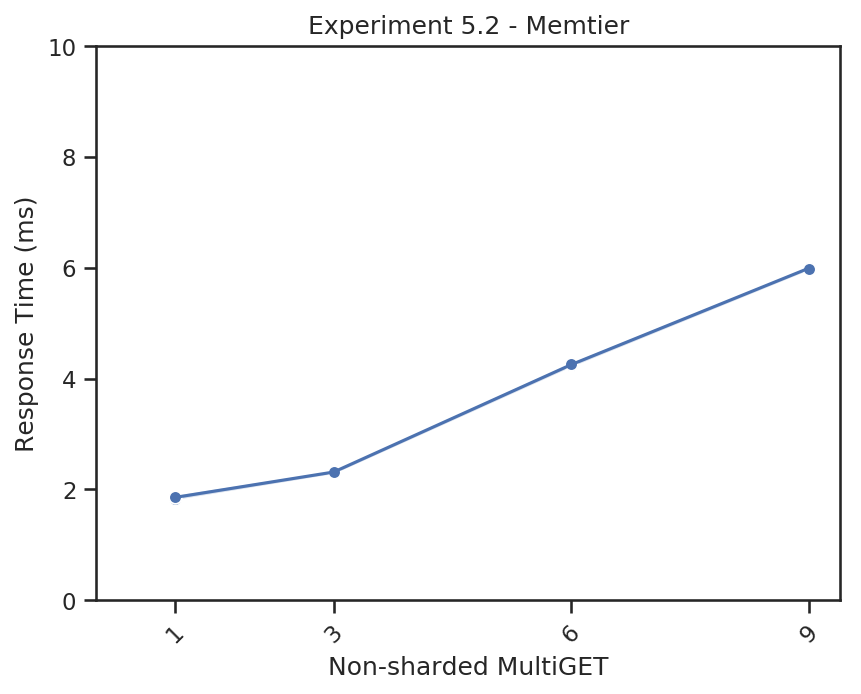
\includegraphics[width=\textwidth]{../data_analysis/figures/5-2_mt_response-time.png}
                \caption{Average response times.\label{fig:noshard_mt_rt}}
            \end{subfigure}
            \begin{subfigure}[t!]{0.56\textwidth}
                \centering
                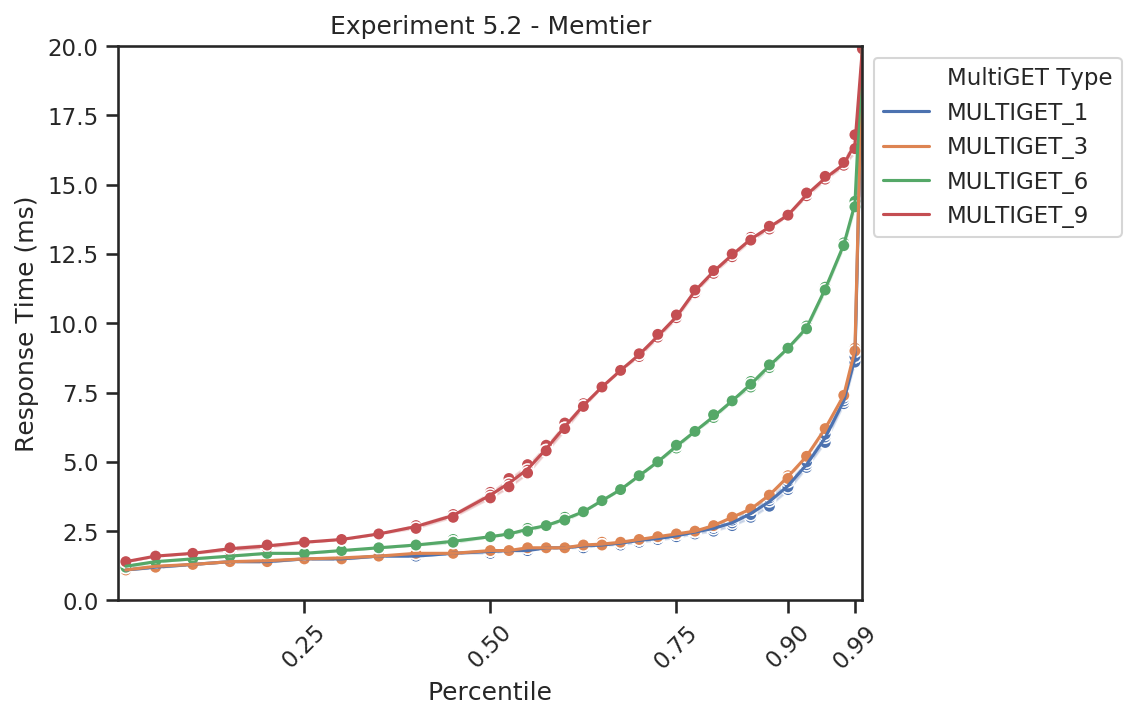
\includegraphics[width=\textwidth]{../data_analysis/figures/5-2_mt_percentiles.png}
                \caption{Percentiles of all response times.\label{fig:noshard_mt_rt_percentiles}}
            \end{subfigure}
            \caption{Response times measured on \cli{}s. The graphs include error bars and represent response times
                     for GET packets using non-sharded behaviour on the \mw.\label{fig:noshard_mt}}
        \end{figure*}

        \begin{figure*}
            \vspace*{-.5\baselineskip}
                \centering
            \begin{subfigure}[t!]{0.48\textwidth}
                \centering
                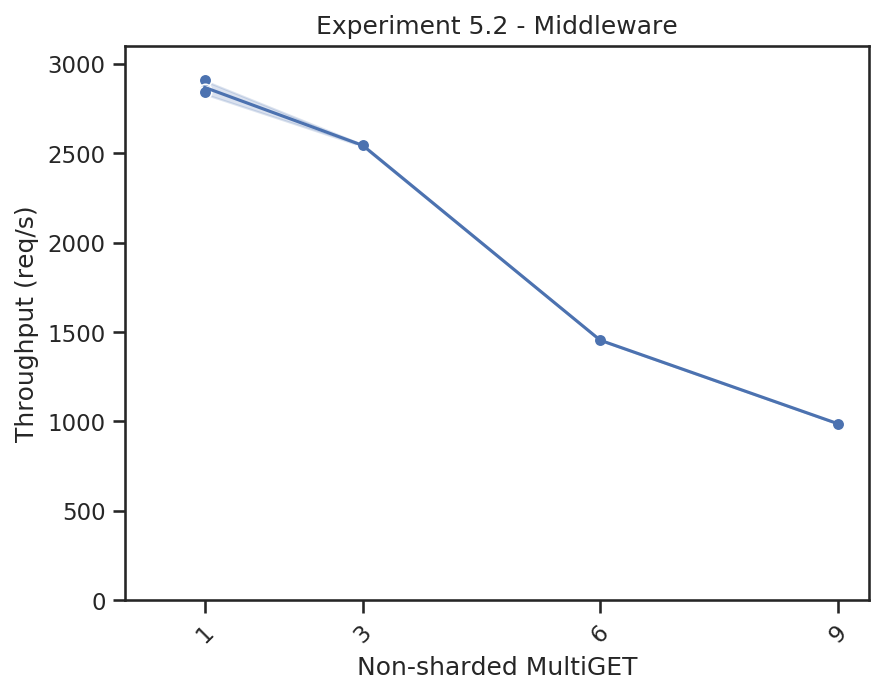
\includegraphics[width=\textwidth]{../data_analysis/figures/5-2_mw_thoughput.png}
                \caption{Request throughput.\label{fig:noshard_mw_tp}}
                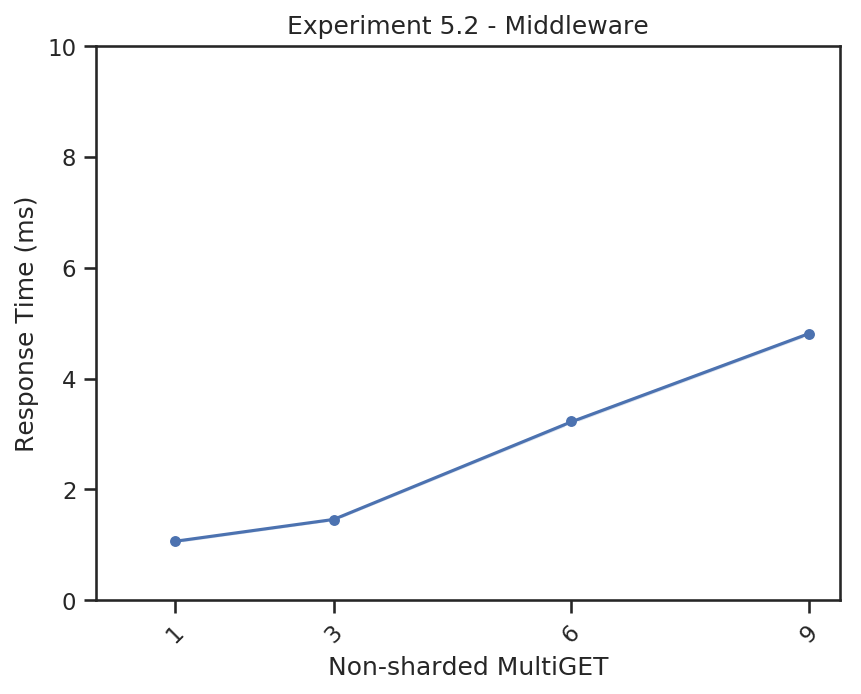
\includegraphics[width=\textwidth]{../data_analysis/figures/5-2_mw_response-time.png}
                \caption{Average response times.\label{fig:noshard_mw_rt}}
            \end{subfigure}
            \begin{subfigure}[t!]{0.48\textwidth}
                \centering
                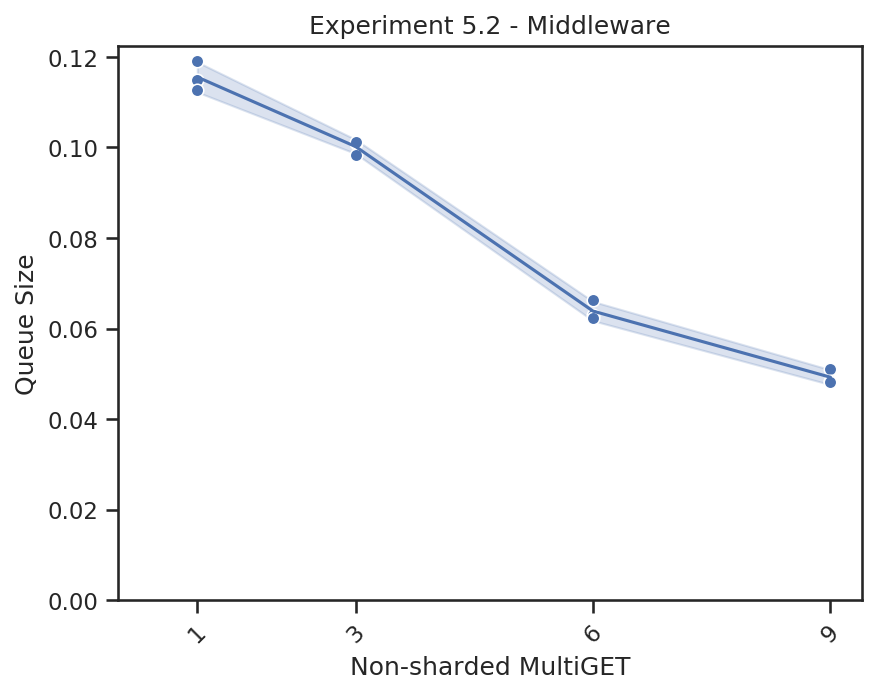
\includegraphics[width=\textwidth]{../data_analysis/figures/5-2_mw_queue-size.png}
                \caption{Queue sizes.\label{fig:noshard_mw_qs}}
                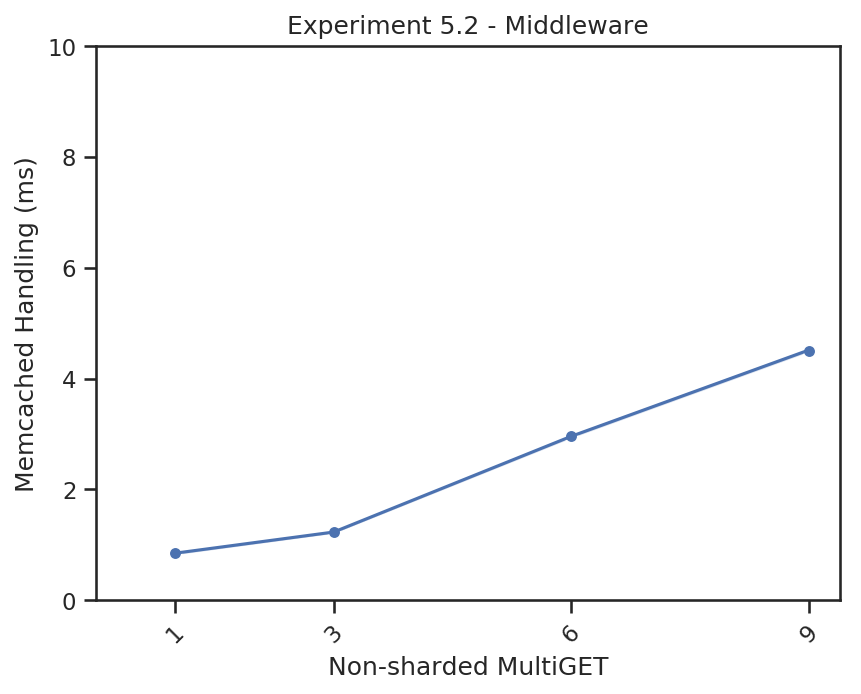
\includegraphics[width=\textwidth]{../data_analysis/figures/5-2_mw_mc-comm-time.png}
                \caption{Memcached communication time.\label{fig:noshard_mw_mct}}
            \end{subfigure}
            \caption{\mw{} statistics based on GET requests. Requests are defined as consisting of one GET request
                     followed by a variable amount of keys to be requested.\label{fig:noshard_mw}}
        \end{figure*}

        \subsubsection{Explanation\label{subsubsec:5_nonsharded_summary}}

            The subfigures of figure \ref{fig:noshard_mt} show similar behaviour to the ones in figure
            \ref{fig:shard_mt}.  Important differences are the decreased 50-percentile point for mutliGETs of size 9
            with higher response times for 6 and 9 keys in the high percentiles. This indicates that sharding helps
            stabilize GET request variance at the cost of a higher average response time. This argument is strengthened
            when comparing the average response times of figures \ref{fig:noshard_mt_rt} and \ref{fig:shard_mt_rt}. For
            non-sharding the average response times are therefore lower (marginally for key sizes below 9) but higher
            variances are to be expected. For both experiments the response time for keys of size 1 are virtually
            identical. This is expected as sharding should not influence this metric.

            % The distribution of percentiles at the 50-percentile matches the average response time graph which is expected.
            % Even though differently sized GET requests are not easily comparable their percentiles grow in a similar
            % fashion. This shows their distributions are all based on the same base model.

            The queue is similarly to the sharded case nearly empty and the middleware spends most of the time
            communicating with a single \srv{} as opposed to multiple ones for GET requests (no sharding occurs). As
            such only a single connection is used which adds the benefit of being able to receive more contiguous data
            from a single connection, meaning more stable behaviour once a replies occurs. This behaviour will be
            compared in subsection \ref{subsec:5_summary}.\newline
            The reported throughput has a slightly stronger bent after 3 keys compared to sharded responses but overall
            the throughputs are comparable between sharded and non-sharded. A closer comparison shows the system
            performing better for GETs with 3 keys and not using sharding (2543 [4] for non-sharded and 2291.64 [12]).
            This reflects back in the percentiles. For the non-sharded case three keys behave extremely similar to a
            single key, whereas this is not the case for the sharded case.

    \subsection{Histogram\label{subsec:5_histograms}}

        \begin{figure*}
            \vspace*{-.5\baselineskip}
                \centering
            \begin{subfigure}[t!]{0.48\textwidth}
                \centering
                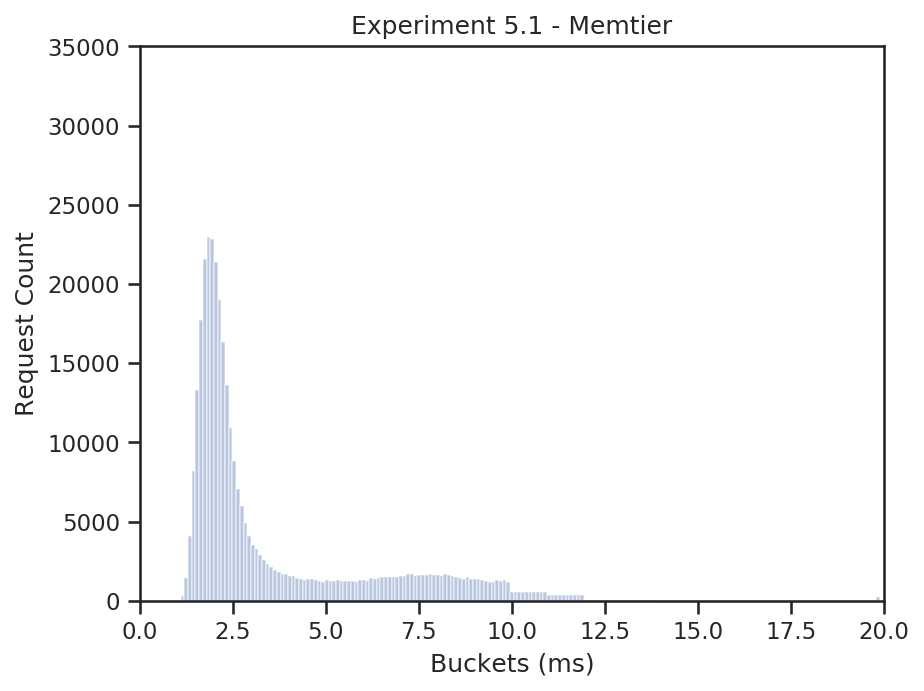
\includegraphics[width=\textwidth]{../data_analysis/figures/5-1_mt_histogram.png}
                \caption{Histogram for sharded multiGET with 6 keys measured on \cli.\label{fig:histogram_sharded_mt}}
                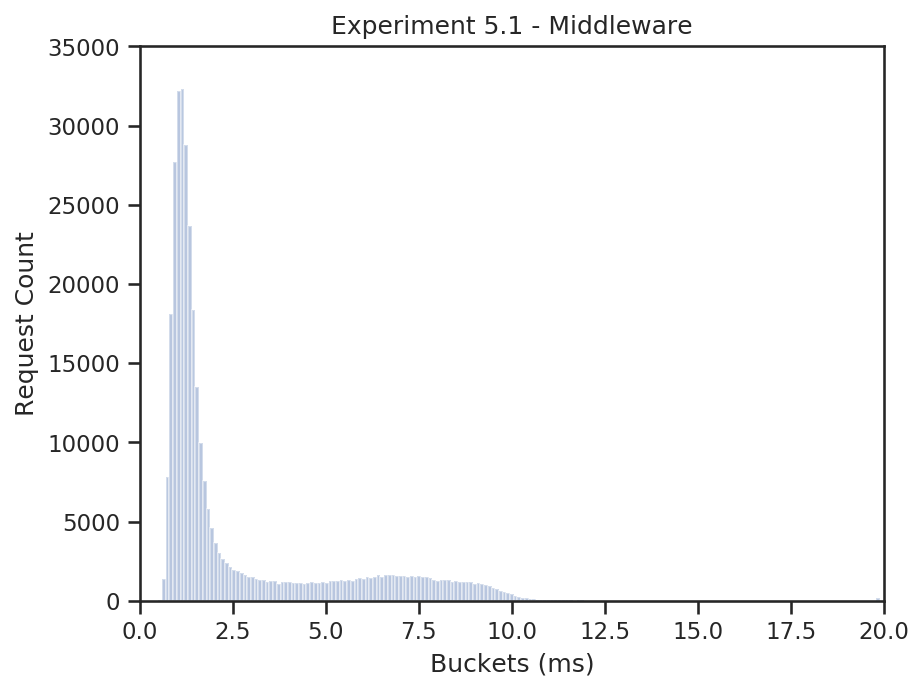
\includegraphics[width=\textwidth]{../data_analysis/figures/5-1_mw_histogram.png}
                \caption{Histogram for sharded multiGET with 6 keys measured on \mw.\label{fig:histogram_sharded_mw}}
            \end{subfigure}
            \begin{subfigure}[t!]{0.48\textwidth}
                \centering
                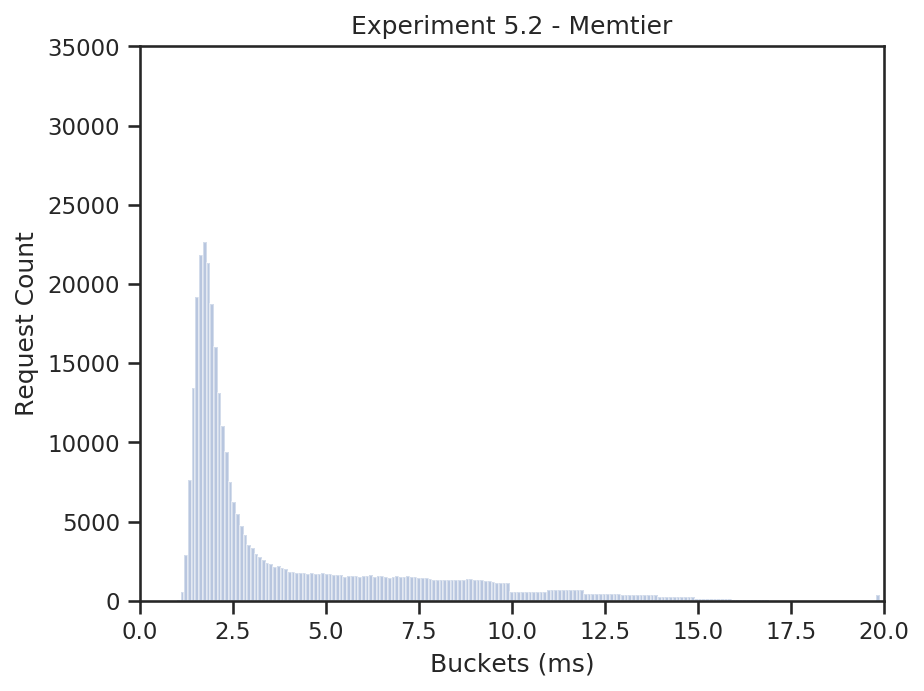
\includegraphics[width=\textwidth]{../data_analysis/figures/5-2_mt_histogram.png}
                \caption{Histogram for non-sharded mutliGET with 6 keys measured on
                \cli.\label{fig:histogram_nonsharded_mt}}
                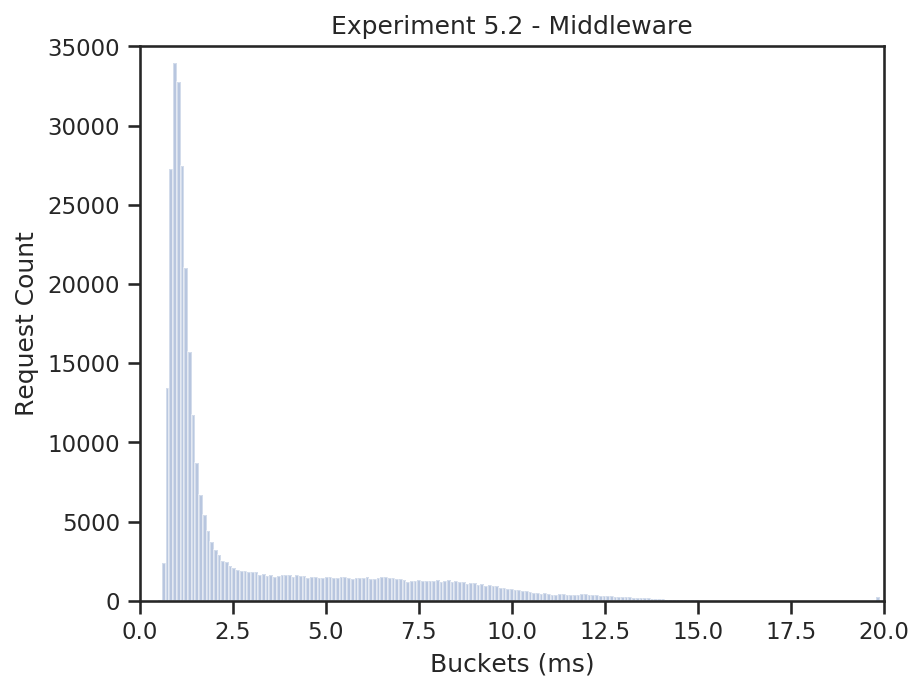
\includegraphics[width=\textwidth]{../data_analysis/figures/5-2_mw_histogram.png}
                \caption{Histogram for non-sharded mutliGET with 6 keys measured on
                \mw.\label{fig:histogram_nonsharded_nw}}
            \end{subfigure}
            \caption{Histograms of response times measured for sharded and non-sharded multiGETs of 6 keys. The
                     distribution is based on GET requests and a bucket sizes of 0.1ms is used, with the last
                     bucket accumulating all values $\geq19.9$ms.\label{fig:histograms}}
        \end{figure*}

        The histograms show consistent behaviour between \srv{}s and \mw{}s; the response times are never smaller for
        \srv{}s than for \mw{}s and the shape measured being smoother on the middleware than on memtier follows from
        a constant bucketing of 0.1ms on the middleware as opposed to memtier which accumulates responses beyond 10ms
        into buckets of 1ms.

        The general shapes are similar between measurements at \mw{}s and \cli{}s for the case of sharded and
        non-sharded multi-key GET requests. The plots for sharding have similar widths and magnitude on the main peak with
        similar tails whereas for the non-sharded case the middleware's main peak is less pronounced compared to memtier
        and slightly wider.

        Noteworthy in figure \ref{fig:histogram_sharded_mw} is the second hill between 7.5\textendash10.0ms. It is
        somewhat visible on the respective \srv{} measurement but doesn't exist for the non-sharded case. This behaviour
        may be due to servers having a variable response time and with each sharded request convolving the expected
        response times from each server for one third of the request size keys. As such the long responses are ``bundled
        up'' and disappear from the observation and slow servers are only expected to send 2 and not 6 keys.

        Additionally the histograms show very few outliers in the last bucket. The represented curves are therefore well
        suited to explain the distribution of response times.

        Lastly the previous claim of sharding increasing the response time yet stabilizing the variance shows well in
        the plots. In general sharded results cut off earlier than the non-sharded counter-part.

    \subsection{Summary\label{subsec:5_summary}}

        The question on how much sharding improves network performance is not easy to answer. Overall the throughput
        stays mostly comparable for GETs with same key sizes.

        The only measurable metric that may be of interest is the reduced response time for the non-sharded case. But
        this only shows significantly for large keys. This seems to indicate that coordinating keys between three
        \srv{}s is more cumbersome than just sending the request to one. Looking at how connection handling and
        memcached communication is designed on the middleware it becomes clear that distributing the GET requests to the
        servers is done quickly. Accepting replies and reassembling the responses is the bottleneck. Even though many
        worker threads exist on the middleware each one handles network communication in a single-threaded approach. As
        such responses begin to be serialized if they arrive simultaneously on the middleware (the thread can only
        handle one connection at a time) and introduce the negative side-effect of requiring more state computations and
        OS-based calls to access data on each of the sockets used for communication. As requests are also guaranteed to
        be over the size of an MTU and the design of network communication returns once no new data is present in the
        socket bad interleavings of accessing partially complete data on sockets introduce further overhead. This
        overhead is not as strongly present for a single connection. Using a single connection introduces the issue of
        two requests being sent to the same \srv{}. As such larger variation is expected as memcached is run single
        threaded.

        In both cases there is a measurable increase in throughput for GET as key increase in size. It approaches the
        upload limit of all three servers. As such the distribution of requests follows a good pattern where the system
        can show its true performance. It becomes clear that increasing the amount of keys per request is therefore one
        way to increase performance for GET requests.

        The interactive law cannot be simply applied to the throughput numbers obtained in figures \ref{fig:shard_mw_tp}
        and \ref{fig:noshard_mw_tp}. Calculating the response time it becomes apparent that the numbers don't match up.
        This stems from the fact that only half the total requests are displayed. The graph only display GET requests,
        not SET requests. As they are send in a 1:1 ratio though, simply by multiplying the amount of requests for
        response time calculation gives a very good approximation of the response time. This response time is then the
        average response time for both GET and SET requests though.

        % Lastly the number of requests may seem low but including the results from experiment \ref{subsec:2_two-servers}
        % it is clear that memtier instances are not saturating memcached and vice-versa. The throughput received
        % therefore is expected to not saturate for GET requests with a single key but more keys add significantly to
        % the throughput of the system.
